\documentclass[1p]{elsarticle_modified}
%\bibliographystyle{elsarticle-num}

%\usepackage[colorlinks]{hyperref}
%\usepackage{abbrmath_seonhwa} %\Abb, \Ascr, \Acal ,\Abf, \Afrak
\usepackage{amsfonts}
\usepackage{amssymb}
\usepackage{amsmath}
\usepackage{amsthm}
\usepackage{scalefnt}
\usepackage{amsbsy}
\usepackage{kotex}
\usepackage{caption}
\usepackage{subfig}
\usepackage{color}
\usepackage{graphicx}
\usepackage{xcolor} %% white, black, red, green, blue, cyan, magenta, yellow
\usepackage{float}
\usepackage{setspace}
\usepackage{hyperref}

\usepackage{tikz}
\usetikzlibrary{arrows}

\usepackage{multirow}
\usepackage{array} % fixed length table
\usepackage{hhline}

%%%%%%%%%%%%%%%%%%%%%
\makeatletter
\renewcommand*\env@matrix[1][\arraystretch]{%
	\edef\arraystretch{#1}%
	\hskip -\arraycolsep
	\let\@ifnextchar\new@ifnextchar
	\array{*\c@MaxMatrixCols c}}
\makeatother %https://tex.stackexchange.com/questions/14071/how-can-i-increase-the-line-spacing-in-a-matrix
%%%%%%%%%%%%%%%

\usepackage[normalem]{ulem}

\newcommand{\msout}[1]{\ifmmode\text{\sout{\ensuremath{#1}}}\else\sout{#1}\fi}
%SOURCE: \msout is \stkout macro in https://tex.stackexchange.com/questions/20609/strikeout-in-math-mode

\newcommand{\cancel}[1]{
	\ifmmode
	{\color{red}\msout{#1}}
	\else
	{\color{red}\sout{#1}}
	\fi
}

\newcommand{\add}[1]{
	{\color{blue}\uwave{#1}}
}

\newcommand{\replace}[2]{
	\ifmmode
	{\color{red}\msout{#1}}{\color{blue}\uwave{#2}}
	\else
	{\color{red}\sout{#1}}{\color{blue}\uwave{#2}}
	\fi
}

\newcommand{\Sol}{\mathcal{S}} %segment
\newcommand{\D}{D} %diagram
\newcommand{\A}{\mathcal{A}} %arc


%%%%%%%%%%%%%%%%%%%%%%%%%%%%%5 test

\def\sl{\operatorname{\textup{SL}}(2,\Cbb)}
\def\psl{\operatorname{\textup{PSL}}(2,\Cbb)}
\def\quan{\mkern 1mu \triangleright \mkern 1mu}

\theoremstyle{definition}
\newtheorem{thm}{Theorem}[section]
\newtheorem{prop}[thm]{Proposition}
\newtheorem{lem}[thm]{Lemma}
\newtheorem{ques}[thm]{Question}
\newtheorem{cor}[thm]{Corollary}
\newtheorem{defn}[thm]{Definition}
\newtheorem{exam}[thm]{Example}
\newtheorem{rmk}[thm]{Remark}
\newtheorem{alg}[thm]{Algorithm}

\newcommand{\I}{\sqrt{-1}}
\begin{document}

%\begin{frontmatter}
%
%\title{Boundary parabolic representations of knots up to 8 crossings}
%
%%% Group authors per affiliation:
%\author{Yunhi Cho} 
%\address{Department of Mathematics, University of Seoul, Seoul, Korea}
%\ead{yhcho@uos.ac.kr}
%
%
%\author{Seonhwa Kim} %\fnref{s_kim}}
%\address{Center for Geometry and Physics, Institute for Basic Science, Pohang, 37673, Korea}
%\ead{ryeona17@ibs.re.kr}
%
%\author{Hyuk Kim}
%\address{Department of Mathematical Sciences, Seoul National University, Seoul 08826, Korea}
%\ead{hyukkim@snu.ac.kr}
%
%\author{Seokbeom Yoon}
%\address{Department of Mathematical Sciences, Seoul National University, Seoul, 08826,  Korea}
%\ead{sbyoon15@snu.ac.kr}
%
%\begin{abstract}
%We find all boundary parabolic representation of knots up to 8 crossings.
%
%\end{abstract}
%\begin{keyword}
%    \MSC[2010] 57M25 
%\end{keyword}
%
%\end{frontmatter}

%\linenumbers
%\tableofcontents
%
\newcommand\colored[1]{\textcolor{white}{\rule[-0.35ex]{0.8em}{1.4ex}}\kern-0.8em\color{red} #1}%
%\newcommand\colored[1]{\textcolor{white}{ #1}\kern-2.17ex	\textcolor{white}{ #1}\kern-1.81ex	\textcolor{white}{ #1}\kern-2.15ex\color{red}#1	}

{\Large $\underline{12n_{0366}~(K12n_{0366})}$}

\setlength{\tabcolsep}{10pt}
\renewcommand{\arraystretch}{1.6}
\vspace{1cm}\begin{tabular}{m{100pt}>{\centering\arraybackslash}m{274pt}}
\multirow{5}{120pt}{
	\centering
	\includegraphics[width=112pt]{../../../GIT/diagram.site/Diagrams/png/2455_12n_0366.png}\\
\ \ \ A knot diagram\footnotemark}&
\allowdisplaybreaks
\textbf{Linearized knot diagam} \\
\cline{2-2}
 &
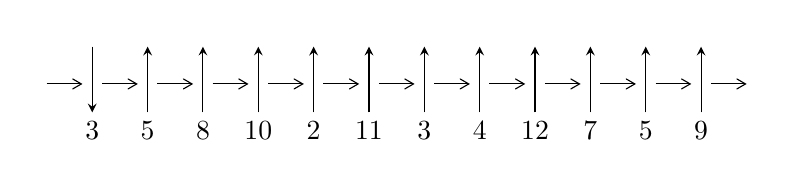
\begin{tikzpicture}[x=20pt, y=17pt]
	% nodes
	\node (C0) at (0, 0) {};
	\node (C1) at (1, 0) {};
	\node (C1U) at (1, +1) {};
	\node (C1D) at (1, -1) {3};

	\node (C2) at (2, 0) {};
	\node (C2U) at (2, +1) {};
	\node (C2D) at (2, -1) {5};

	\node (C3) at (3, 0) {};
	\node (C3U) at (3, +1) {};
	\node (C3D) at (3, -1) {8};

	\node (C4) at (4, 0) {};
	\node (C4U) at (4, +1) {};
	\node (C4D) at (4, -1) {10};

	\node (C5) at (5, 0) {};
	\node (C5U) at (5, +1) {};
	\node (C5D) at (5, -1) {2};

	\node (C6) at (6, 0) {};
	\node (C6U) at (6, +1) {};
	\node (C6D) at (6, -1) {11};

	\node (C7) at (7, 0) {};
	\node (C7U) at (7, +1) {};
	\node (C7D) at (7, -1) {3};

	\node (C8) at (8, 0) {};
	\node (C8U) at (8, +1) {};
	\node (C8D) at (8, -1) {4};

	\node (C9) at (9, 0) {};
	\node (C9U) at (9, +1) {};
	\node (C9D) at (9, -1) {12};

	\node (C10) at (10, 0) {};
	\node (C10U) at (10, +1) {};
	\node (C10D) at (10, -1) {7};

	\node (C11) at (11, 0) {};
	\node (C11U) at (11, +1) {};
	\node (C11D) at (11, -1) {5};

	\node (C12) at (12, 0) {};
	\node (C12U) at (12, +1) {};
	\node (C12D) at (12, -1) {9};
	\node (C13) at (13, 0) {};

	% arrows
	\draw[->,>={angle 60}]
	(C0) edge (C1) (C1) edge (C2) (C2) edge (C3) (C3) edge (C4) (C4) edge (C5) (C5) edge (C6) (C6) edge (C7) (C7) edge (C8) (C8) edge (C9) (C9) edge (C10) (C10) edge (C11) (C11) edge (C12) (C12) edge (C13) ;	\draw[->,>=stealth]
	(C1U) edge (C1D) (C2D) edge (C2U) (C3D) edge (C3U) (C4D) edge (C4U) (C5D) edge (C5U) (C6D) edge (C6U) (C7D) edge (C7U) (C8D) edge (C8U) (C9D) edge (C9U) (C10D) edge (C10U) (C11D) edge (C11U) (C12D) edge (C12U) ;
	\end{tikzpicture} \\
\hhline{~~} \\& 
\textbf{Solving Sequence} \\ \cline{2-2} 
 &
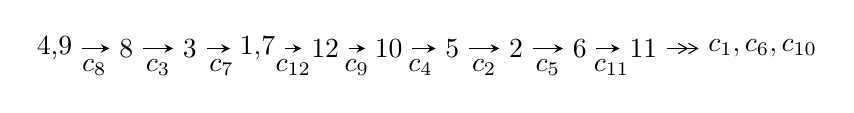
\begin{tikzpicture}[x=23pt, y=7pt]
	% node
	\node (A0) at (-1/8, 0) {4,9};
	\node (A1) at (1, 0) {8};
	\node (A2) at (2, 0) {3};
	\node (A3) at (49/16, 0) {1,7};
	\node (A4) at (33/8, 0) {12};
	\node (A5) at (41/8, 0) {10};
	\node (A6) at (49/8, 0) {5};
	\node (A7) at (57/8, 0) {2};
	\node (A8) at (65/8, 0) {6};
	\node (A9) at (73/8, 0) {11};
	\node (C1) at (1/2, -1) {$c_{8}$};
	\node (C2) at (3/2, -1) {$c_{3}$};
	\node (C3) at (5/2, -1) {$c_{7}$};
	\node (C4) at (29/8, -1) {$c_{12}$};
	\node (C5) at (37/8, -1) {$c_{9}$};
	\node (C6) at (45/8, -1) {$c_{4}$};
	\node (C7) at (53/8, -1) {$c_{2}$};
	\node (C8) at (61/8, -1) {$c_{5}$};
	\node (C9) at (69/8, -1) {$c_{11}$};
	\node (A10) at (11, 0) {$c_{1},c_{6},c_{10}$};

	% edge
	\draw[->,>=stealth]	
	(A0) edge (A1) (A1) edge (A2) (A2) edge (A3) (A3) edge (A4) (A4) edge (A5) (A5) edge (A6) (A6) edge (A7) (A7) edge (A8) (A8) edge (A9) ;
	\draw[->>,>={angle 60}]	
	(A9) edge (A10);
\end{tikzpicture} \\ 

\end{tabular} \\

\footnotetext{
The image of knot diagram is generated by the software ``\textbf{Draw programme}" developed by Andrew Bartholomew(\url{http://www.layer8.co.uk/maths/draw/index.htm\#Running-draw}), where we modified some parts for our purpose(\url{https://github.com/CATsTAILs/LinksPainter}).
}\phantom \\ \newline 
\centering \textbf{Ideals for irreducible components\footnotemark of $X_{\text{par}}$} 
 
\begin{align*}
I^u_{1}&=\langle 
8.60410\times10^{36} u^{33}-9.82765\times10^{36} u^{32}+\cdots+2.12256\times10^{38} b+1.92039\times10^{38},\\
\phantom{I^u_{1}}&\phantom{= \langle  }3.53556\times10^{37} u^{33}+3.38592\times10^{37} u^{32}+\cdots+8.49024\times10^{38} a-2.51443\times10^{39},\;u^{34}- u^{33}+\cdots+14 u-4\rangle \\
I^u_{2}&=\langle 
-41317 u^{19}+14868 u^{18}+\cdots+102043 b-217021,\\
\phantom{I^u_{2}}&\phantom{= \langle  }-20816 u^{19}+54137 u^{18}+\cdots+204086 a+123227,\;u^{20}-10 u^{18}+\cdots+6 u+4\rangle \\
\\
\end{align*}
\raggedright * 2 irreducible components of $\dim_{\mathbb{C}}=0$, with total 54 representations.\\
\footnotetext{All coefficients of polynomials are rational numbers. But the coefficients are sometimes approximated in decimal forms when there is not enough margin.}
\newpage
\renewcommand{\arraystretch}{1}
\centering \section*{I. $I^u_{1}= \langle 8.60\times10^{36} u^{33}-9.83\times10^{36} u^{32}+\cdots+2.12\times10^{38} b+1.92\times10^{38},\;3.54\times10^{37} u^{33}+3.39\times10^{37} u^{32}+\cdots+8.49\times10^{38} a-2.51\times10^{39},\;u^{34}- u^{33}+\cdots+14 u-4 \rangle$}
\flushleft \textbf{(i) Arc colorings}\\
\begin{tabular}{m{7pt} m{180pt} m{7pt} m{180pt} }
\flushright $a_{4}=$&$\begin{pmatrix}0\\u\end{pmatrix}$ \\
\flushright $a_{9}=$&$\begin{pmatrix}1\\0\end{pmatrix}$ \\
\flushright $a_{8}=$&$\begin{pmatrix}1\\u^2\end{pmatrix}$ \\
\flushright $a_{3}=$&$\begin{pmatrix}- u\\- u^3+u\end{pmatrix}$ \\
\flushright $a_{1}=$&$\begin{pmatrix}-0.0416427 u^{33}-0.0398802 u^{32}+\cdots+1.58286 u+2.96155\\-0.0405364 u^{33}+0.0463009 u^{32}+\cdots+1.98650 u-0.904754\end{pmatrix}$ \\
\flushright $a_{7}=$&$\begin{pmatrix}- u^2+1\\- u^4+2 u^2\end{pmatrix}$ \\
\flushright $a_{12}=$&$\begin{pmatrix}-0.00110628 u^{33}-0.0861811 u^{32}+\cdots-0.403640 u+3.86631\\-0.0405364 u^{33}+0.0463009 u^{32}+\cdots+1.98650 u-0.904754\end{pmatrix}$ \\
\flushright $a_{10}=$&$\begin{pmatrix}0.322523 u^{33}-0.187269 u^{32}+\cdots-12.1237 u+3.64934\\-0.0561189 u^{33}+0.0359757 u^{32}+\cdots+2.41252 u-0.0498318\end{pmatrix}$ \\
\flushright $a_{5}=$&$\begin{pmatrix}0.309604 u^{33}-0.157316 u^{32}+\cdots-11.9411 u+1.11047\\-0.115816 u^{33}-0.0301325 u^{32}+\cdots+2.98843 u+0.206879\end{pmatrix}$ \\
\flushright $a_{2}=$&$\begin{pmatrix}0.0473120 u^{33}-0.0631917 u^{32}+\cdots+0.283713 u+3.39961\\-0.0678345 u^{33}+0.0620244 u^{32}+\cdots+2.72246 u-1.08024\end{pmatrix}$ \\
\flushright $a_{6}=$&$\begin{pmatrix}-0.00781040 u^{33}+0.0389021 u^{32}+\cdots-0.701468 u-1.89917\\-0.203245 u^{33}-0.107497 u^{32}+\cdots+1.28592 u-0.355887\end{pmatrix}$ \\
\flushright $a_{11}=$&$\begin{pmatrix}0.361377 u^{33}-0.196045 u^{32}+\cdots-11.6891 u+3.77920\\-0.219182 u^{33}+0.0237395 u^{32}+\cdots+3.96379 u-0.616850\end{pmatrix}$\\&\end{tabular}
\flushleft \textbf{(ii) Obstruction class $= -1$}\\~\\
\flushleft \textbf{(iii) Cusp Shapes $= 0.349003 u^{33}+0.651298 u^{32}+\cdots-1.59052 u+10.7798$}\\~\\
\newpage\renewcommand{\arraystretch}{1}
\flushleft \textbf{(iv) u-Polynomials at the component}\newline \\
\begin{tabular}{m{50pt}|m{274pt}}
Crossings & \hspace{64pt}u-Polynomials at each crossing \\
\hline $$\begin{aligned}c_{1}\end{aligned}$$&$\begin{aligned}
&u^{34}+52 u^{33}+\cdots-125583 u+7921
\end{aligned}$\\
\hline $$\begin{aligned}c_{2},c_{5}\end{aligned}$$&$\begin{aligned}
&u^{34}+2 u^{33}+\cdots+91 u+89
\end{aligned}$\\
\hline $$\begin{aligned}c_{3},c_{7},c_{8}\end{aligned}$$&$\begin{aligned}
&u^{34}+u^{33}+\cdots-14 u-4
\end{aligned}$\\
\hline $$\begin{aligned}c_{4}\end{aligned}$$&$\begin{aligned}
&u^{34}- u^{33}+\cdots-1046 u-137
\end{aligned}$\\
\hline $$\begin{aligned}c_{6},c_{10}\end{aligned}$$&$\begin{aligned}
&u^{34}- u^{33}+\cdots+75 u+17
\end{aligned}$\\
\hline $$\begin{aligned}c_{9},c_{12}\end{aligned}$$&$\begin{aligned}
&u^{34}+3 u^{33}+\cdots+11 u+1
\end{aligned}$\\
\hline $$\begin{aligned}c_{11}\end{aligned}$$&$\begin{aligned}
&u^{34}+u^{33}+\cdots-5852 u+764
\end{aligned}$\\
\hline
\end{tabular}\\~\\
\newpage\renewcommand{\arraystretch}{1}
\flushleft \textbf{(v) Riley Polynomials at the component}\newline \\
\begin{tabular}{m{50pt}|m{274pt}}
Crossings & \hspace{64pt}Riley Polynomials at each crossing \\
\hline $$\begin{aligned}c_{1}\end{aligned}$$&$\begin{aligned}
&y^{34}-152 y^{33}+\cdots-3985291411 y+62742241
\end{aligned}$\\
\hline $$\begin{aligned}c_{2},c_{5}\end{aligned}$$&$\begin{aligned}
&y^{34}+52 y^{33}+\cdots-125583 y+7921
\end{aligned}$\\
\hline $$\begin{aligned}c_{3},c_{7},c_{8}\end{aligned}$$&$\begin{aligned}
&y^{34}-23 y^{33}+\cdots-140 y+16
\end{aligned}$\\
\hline $$\begin{aligned}c_{4}\end{aligned}$$&$\begin{aligned}
&y^{34}+11 y^{33}+\cdots-925058 y+18769
\end{aligned}$\\
\hline $$\begin{aligned}c_{6},c_{10}\end{aligned}$$&$\begin{aligned}
&y^{34}+57 y^{33}+\cdots-16675 y+289
\end{aligned}$\\
\hline $$\begin{aligned}c_{9},c_{12}\end{aligned}$$&$\begin{aligned}
&y^{34}+25 y^{33}+\cdots+223 y+1
\end{aligned}$\\
\hline $$\begin{aligned}c_{11}\end{aligned}$$&$\begin{aligned}
&y^{34}+73 y^{33}+\cdots+16521896 y+583696
\end{aligned}$\\
\hline
\end{tabular}\\~\\
\newpage\flushleft \textbf{(vi) Complex Volumes and Cusp Shapes}
$$\begin{array}{c|c|c}  
\text{Solutions to }I^u_{1}& \I (\text{vol} + \sqrt{-1}CS) & \text{Cusp shape}\\
 \hline 
\begin{aligned}
u &= -0.922036 + 0.452881 I \\
a &= -1.95374 + 1.73996 I \\
b &= \phantom{-}0.050107 - 0.380343 I\end{aligned}
 & -10.10770 - 1.83068 I & -1.32953 + 4.89170 I \\ \hline\begin{aligned}
u &= -0.922036 - 0.452881 I \\
a &= -1.95374 - 1.73996 I \\
b &= \phantom{-}0.050107 + 0.380343 I\end{aligned}
 & -10.10770 + 1.83068 I & -1.32953 - 4.89170 I \\ \hline\begin{aligned}
u &= \phantom{-}1.06806\phantom{ +0.000000I} \\
a &= -1.57173\phantom{ +0.000000I} \\
b &= -1.48329\phantom{ +0.000000I}\end{aligned}
 & \phantom{-}5.61986\phantom{ +0.000000I} & \phantom{-}15.0470\phantom{ +0.000000I} \\ \hline\begin{aligned}
u &= -0.684975 + 0.829271 I \\
a &= \phantom{-}1.26384 - 0.77066 I \\
b &= \phantom{-}0.61689 - 1.83184 I\end{aligned}
 & -6.65191 - 3.35398 I & \phantom{-}5.96369 + 3.28451 I \\ \hline\begin{aligned}
u &= -0.684975 - 0.829271 I \\
a &= \phantom{-}1.26384 + 0.77066 I \\
b &= \phantom{-}0.61689 + 1.83184 I\end{aligned}
 & -6.65191 + 3.35398 I & \phantom{-}5.96369 - 3.28451 I \\ \hline\begin{aligned}
u &= \phantom{-}0.737579 + 0.460594 I \\
a &= -0.619611 + 0.405450 I \\
b &= \phantom{-}0.306540 - 0.990036 I\end{aligned}
 & -4.82144 - 1.46148 I & \phantom{-}3.54664 - 1.80098 I \\ \hline\begin{aligned}
u &= \phantom{-}0.737579 - 0.460594 I \\
a &= -0.619611 - 0.405450 I \\
b &= \phantom{-}0.306540 + 0.990036 I\end{aligned}
 & -4.82144 + 1.46148 I & \phantom{-}3.54664 + 1.80098 I \\ \hline\begin{aligned}
u &= -1.123130 + 0.394227 I \\
a &= \phantom{-}1.244230 - 0.472944 I \\
b &= \phantom{-}0.304757 - 1.086760 I\end{aligned}
 & \phantom{-}0.20788 - 1.57648 I & \phantom{-}10.97463 + 0.65835 I \\ \hline\begin{aligned}
u &= -1.123130 - 0.394227 I \\
a &= \phantom{-}1.244230 + 0.472944 I \\
b &= \phantom{-}0.304757 + 1.086760 I\end{aligned}
 & \phantom{-}0.20788 + 1.57648 I & \phantom{-}10.97463 - 0.65835 I \\ \hline\begin{aligned}
u &= \phantom{-}0.929580 + 0.767374 I \\
a &= \phantom{-}2.11679 - 0.95570 I \\
b &= \phantom{-}1.91672 - 0.56786 I\end{aligned}
 & -12.29770 + 2.91676 I & \phantom{-}6.61132 - 2.45322 I\\
 \hline 
 \end{array}$$\newpage$$\begin{array}{c|c|c}  
\text{Solutions to }I^u_{1}& \I (\text{vol} + \sqrt{-1}CS) & \text{Cusp shape}\\
 \hline 
\begin{aligned}
u &= \phantom{-}0.929580 - 0.767374 I \\
a &= \phantom{-}2.11679 + 0.95570 I \\
b &= \phantom{-}1.91672 + 0.56786 I\end{aligned}
 & -12.29770 - 2.91676 I & \phantom{-}6.61132 + 2.45322 I \\ \hline\begin{aligned}
u &= \phantom{-}1.21069\phantom{ +0.000000I} \\
a &= -2.25852\phantom{ +0.000000I} \\
b &= -1.75624\phantom{ +0.000000I}\end{aligned}
 & \phantom{-}6.57930\phantom{ +0.000000I} & \phantom{-}4.63880\phantom{ +0.000000I} \\ \hline\begin{aligned}
u &= \phantom{-}1.083810 + 0.540124 I \\
a &= \phantom{-}1.67600 + 0.04657 I \\
b &= \phantom{-}0.496553 + 0.990924 I\end{aligned}
 & -3.48312 + 5.52227 I & \phantom{-}3.76620 - 5.89114 I \\ \hline\begin{aligned}
u &= \phantom{-}1.083810 - 0.540124 I \\
a &= \phantom{-}1.67600 - 0.04657 I \\
b &= \phantom{-}0.496553 - 0.990924 I\end{aligned}
 & -3.48312 - 5.52227 I & \phantom{-}3.76620 + 5.89114 I \\ \hline\begin{aligned}
u &= \phantom{-}1.25801\phantom{ +0.000000I} \\
a &= -1.22256\phantom{ +0.000000I} \\
b &= -1.08785\phantom{ +0.000000I}\end{aligned}
 & \phantom{-}5.55227\phantom{ +0.000000I} & \phantom{-}15.4310\phantom{ +0.000000I} \\ \hline\begin{aligned}
u &= \phantom{-}0.553050 + 0.482320 I \\
a &= \phantom{-}0.680935 - 0.534063 I \\
b &= \phantom{-}0.442741 - 0.243060 I\end{aligned}
 & -2.01055 + 1.80457 I & \phantom{-}7.37027 - 4.67563 I \\ \hline\begin{aligned}
u &= \phantom{-}0.553050 - 0.482320 I \\
a &= \phantom{-}0.680935 + 0.534063 I \\
b &= \phantom{-}0.442741 + 0.243060 I\end{aligned}
 & -2.01055 - 1.80457 I & \phantom{-}7.37027 + 4.67563 I \\ \hline\begin{aligned}
u &= -0.399666 + 0.569326 I \\
a &= -1.124570 - 0.795239 I \\
b &= -0.495351 + 1.172960 I\end{aligned}
 & -2.05097 - 2.54093 I & \phantom{-}8.54961 + 2.56274 I \\ \hline\begin{aligned}
u &= -0.399666 - 0.569326 I \\
a &= -1.124570 + 0.795239 I \\
b &= -0.495351 - 1.172960 I\end{aligned}
 & -2.05097 + 2.54093 I & \phantom{-}8.54961 - 2.56274 I \\ \hline\begin{aligned}
u &= \phantom{-}1.271090 + 0.324893 I \\
a &= -1.326110 - 0.185075 I \\
b &= -0.562882 - 1.237790 I\end{aligned}
 & \phantom{-}1.94144 + 5.55900 I & \phantom{-}17.2677 - 4.1054 I\\
 \hline 
 \end{array}$$\newpage$$\begin{array}{c|c|c}  
\text{Solutions to }I^u_{1}& \I (\text{vol} + \sqrt{-1}CS) & \text{Cusp shape}\\
 \hline 
\begin{aligned}
u &= \phantom{-}1.271090 - 0.324893 I \\
a &= -1.326110 + 0.185075 I \\
b &= -0.562882 + 1.237790 I\end{aligned}
 & \phantom{-}1.94144 - 5.55900 I & \phantom{-}17.2677 + 4.1054 I \\ \hline\begin{aligned}
u &= -1.133490 + 0.786019 I \\
a &= -1.17308 + 1.24490 I \\
b &= -0.45959 + 1.84212 I\end{aligned}
 & -5.26755 - 2.76815 I & \phantom{-}6.74305 + 1.96876 I \\ \hline\begin{aligned}
u &= -1.133490 - 0.786019 I \\
a &= -1.17308 - 1.24490 I \\
b &= -0.45959 - 1.84212 I\end{aligned}
 & -5.26755 + 2.76815 I & \phantom{-}6.74305 - 1.96876 I \\ \hline\begin{aligned}
u &= \phantom{-}0.088561 + 1.396340 I \\
a &= \phantom{-}0.226588 - 0.656943 I \\
b &= \phantom{-}0.51304 - 1.81326 I\end{aligned}
 & \phantom{-}19.1288 - 5.4062 I & \phantom{-}6.05474 + 2.05125 I \\ \hline\begin{aligned}
u &= \phantom{-}0.088561 - 1.396340 I \\
a &= \phantom{-}0.226588 + 0.656943 I \\
b &= \phantom{-}0.51304 + 1.81326 I\end{aligned}
 & \phantom{-}19.1288 + 5.4062 I & \phantom{-}6.05474 - 2.05125 I \\ \hline\begin{aligned}
u &= -1.51491 + 0.11448 I \\
a &= \phantom{-}0.207183 + 0.310262 I \\
b &= \phantom{-}0.0322077 - 0.0682113 I\end{aligned}
 & \phantom{-}4.60570 - 3.56043 I & \phantom{-}15.4789 + 7.9563 I \\ \hline\begin{aligned}
u &= -1.51491 - 0.11448 I \\
a &= \phantom{-}0.207183 - 0.310262 I \\
b &= \phantom{-}0.0322077 + 0.0682113 I\end{aligned}
 & \phantom{-}4.60570 + 3.56043 I & \phantom{-}15.4789 - 7.9563 I \\ \hline\begin{aligned}
u &= \phantom{-}1.47491 + 0.70325 I \\
a &= \phantom{-}1.73912 + 0.75900 I \\
b &= \phantom{-}0.93744 + 1.60343 I\end{aligned}
 & -16.0299 + 12.7557 I & \phantom{-}10.00000 - 5.13495 I \\ \hline\begin{aligned}
u &= \phantom{-}1.47491 - 0.70325 I \\
a &= \phantom{-}1.73912 - 0.75900 I \\
b &= \phantom{-}0.93744 - 1.60343 I\end{aligned}
 & -16.0299 - 12.7557 I & \phantom{-}10.00000 + 5.13495 I \\ \hline\begin{aligned}
u &= -0.345078\phantom{ +0.000000I} \\
a &= \phantom{-}0.490141\phantom{ +0.000000I} \\
b &= -0.241609\phantom{ +0.000000I}\end{aligned}
 & \phantom{-}0.549407\phantom{ +0.000000I} & \phantom{-}18.2220\phantom{ +0.000000I}\\
 \hline 
 \end{array}$$\newpage$$\begin{array}{c|c|c}  
\text{Solutions to }I^u_{1}& \I (\text{vol} + \sqrt{-1}CS) & \text{Cusp shape}\\
 \hline 
\begin{aligned}
u &= \phantom{-}0.169258 + 0.230162 I \\
a &= \phantom{-}3.30928 - 1.57909 I \\
b &= -0.261095 + 0.870304 I\end{aligned}
 & -1.73764 - 2.47115 I & \phantom{-}11.65169 + 4.43713 I \\ \hline\begin{aligned}
u &= \phantom{-}0.169258 - 0.230162 I \\
a &= \phantom{-}3.30928 + 1.57909 I \\
b &= -0.261095 - 0.870304 I\end{aligned}
 & -1.73764 + 2.47115 I & \phantom{-}11.65169 - 4.43713 I \\ \hline\begin{aligned}
u &= -1.62548 + 0.63340 I \\
a &= -0.73552 + 1.36542 I \\
b &= -0.05359 + 1.57787 I\end{aligned}
 & -14.9890 - 1.9387 I & \phantom{-0.000000 } 0 \\ \hline\begin{aligned}
u &= -1.62548 - 0.63340 I \\
a &= -0.73552 - 1.36542 I \\
b &= -0.05359 - 1.57787 I\end{aligned}
 & -14.9890 + 1.9387 I & \phantom{-0.000000 } 0\\
 \hline 
 \end{array}$$\newpage\newpage\renewcommand{\arraystretch}{1}
\centering \section*{II. $I^u_{2}= \langle -4.13\times10^{4} u^{19}+1.49\times10^{4} u^{18}+\cdots+1.02\times10^{5} b-2.17\times10^{5},\;-2.08\times10^{4} u^{19}+5.41\times10^{4} u^{18}+\cdots+2.04\times10^{5} a+1.23\times10^{5},\;u^{20}-10 u^{18}+\cdots+6 u+4 \rangle$}
\flushleft \textbf{(i) Arc colorings}\\
\begin{tabular}{m{7pt} m{180pt} m{7pt} m{180pt} }
\flushright $a_{4}=$&$\begin{pmatrix}0\\u\end{pmatrix}$ \\
\flushright $a_{9}=$&$\begin{pmatrix}1\\0\end{pmatrix}$ \\
\flushright $a_{8}=$&$\begin{pmatrix}1\\u^2\end{pmatrix}$ \\
\flushright $a_{3}=$&$\begin{pmatrix}- u\\- u^3+u\end{pmatrix}$ \\
\flushright $a_{1}=$&$\begin{pmatrix}0.101996 u^{19}-0.265266 u^{18}+\cdots-1.49571 u-0.603799\\0.404898 u^{19}-0.145703 u^{18}+\cdots-2.53587 u+2.12676\end{pmatrix}$ \\
\flushright $a_{7}=$&$\begin{pmatrix}- u^2+1\\- u^4+2 u^2\end{pmatrix}$ \\
\flushright $a_{12}=$&$\begin{pmatrix}-0.302902 u^{19}-0.119562 u^{18}+\cdots+1.04016 u-2.73056\\0.404898 u^{19}-0.145703 u^{18}+\cdots-2.53587 u+2.12676\end{pmatrix}$ \\
\flushright $a_{10}=$&$\begin{pmatrix}0.992150 u^{19}-0.400944 u^{18}+\cdots-2.37768 u+4.62098\\-0.0780847 u^{19}-0.198152 u^{18}+\cdots-3.56977 u-1.72914\end{pmatrix}$ \\
\flushright $a_{5}=$&$\begin{pmatrix}-0.501860 u^{19}+0.227585 u^{18}+\cdots-1.29265 u-2.70449\\-0.400944 u^{19}-0.417304 u^{18}+\cdots+6.66808 u+0.0313985\end{pmatrix}$ \\
\flushright $a_{2}=$&$\begin{pmatrix}0.0242741 u^{19}-0.129666 u^{18}+\cdots+0.735984 u-0.802951\\0.810158 u^{19}+0.0423449 u^{18}+\cdots-5.27028 u+1.78351\end{pmatrix}$ \\
\flushright $a_{6}=$&$\begin{pmatrix}-0.554884 u^{19}-0.0858119 u^{18}+\cdots+1.98350 u+0.737253\\-1.23375 u^{19}-0.323609 u^{18}+\cdots+12.8278 u+0.0295856\end{pmatrix}$ \\
\flushright $a_{11}=$&$\begin{pmatrix}0.664975 u^{19}-0.390840 u^{18}+\cdots-3.07351 u+2.69337\\-0.414012 u^{19}+0.324383 u^{18}+\cdots-4.90638 u-4.90765\end{pmatrix}$\\&\end{tabular}
\flushleft \textbf{(ii) Obstruction class $= 1$}\\~\\
\flushleft \textbf{(iii) Cusp Shapes $= \frac{150899}{102043} u^{19}+\frac{457156}{102043} u^{18}+\cdots-\frac{3098728}{102043} u-\frac{1725625}{102043}$}\\~\\
\newpage\renewcommand{\arraystretch}{1}
\flushleft \textbf{(iv) u-Polynomials at the component}\newline \\
\begin{tabular}{m{50pt}|m{274pt}}
Crossings & \hspace{64pt}u-Polynomials at each crossing \\
\hline $$\begin{aligned}c_{1}\end{aligned}$$&$\begin{aligned}
&u^{20}-15 u^{19}+\cdots-10 u+1
\end{aligned}$\\
\hline $$\begin{aligned}c_{2}\end{aligned}$$&$\begin{aligned}
&u^{20}+u^{19}+\cdots+2 u-1
\end{aligned}$\\
\hline $$\begin{aligned}c_{3}\end{aligned}$$&$\begin{aligned}
&u^{20}-10 u^{18}+\cdots-6 u+4
\end{aligned}$\\
\hline $$\begin{aligned}c_{4}\end{aligned}$$&$\begin{aligned}
&u^{20}-3 u^{18}+\cdots+u-1
\end{aligned}$\\
\hline $$\begin{aligned}c_{5}\end{aligned}$$&$\begin{aligned}
&u^{20}- u^{19}+\cdots-2 u-1
\end{aligned}$\\
\hline $$\begin{aligned}c_{6}\end{aligned}$$&$\begin{aligned}
&u^{20}+8 u^{18}+\cdots-2 u-1
\end{aligned}$\\
\hline $$\begin{aligned}c_{7},c_{8}\end{aligned}$$&$\begin{aligned}
&u^{20}-10 u^{18}+\cdots+6 u+4
\end{aligned}$\\
\hline $$\begin{aligned}c_{9}\end{aligned}$$&$\begin{aligned}
&u^{20}+4 u^{19}+\cdots+6 u^2+1
\end{aligned}$\\
\hline $$\begin{aligned}c_{10}\end{aligned}$$&$\begin{aligned}
&u^{20}+8 u^{18}+\cdots+2 u-1
\end{aligned}$\\
\hline $$\begin{aligned}c_{11}\end{aligned}$$&$\begin{aligned}
&u^{20}+6 u^{18}+\cdots-20 u-112
\end{aligned}$\\
\hline $$\begin{aligned}c_{12}\end{aligned}$$&$\begin{aligned}
&u^{20}-4 u^{19}+\cdots+6 u^2+1
\end{aligned}$\\
\hline
\end{tabular}\\~\\
\newpage\renewcommand{\arraystretch}{1}
\flushleft \textbf{(v) Riley Polynomials at the component}\newline \\
\begin{tabular}{m{50pt}|m{274pt}}
Crossings & \hspace{64pt}Riley Polynomials at each crossing \\
\hline $$\begin{aligned}c_{1}\end{aligned}$$&$\begin{aligned}
&y^{20}-33 y^{19}+\cdots+22 y+1
\end{aligned}$\\
\hline $$\begin{aligned}c_{2},c_{5}\end{aligned}$$&$\begin{aligned}
&y^{20}+15 y^{19}+\cdots+10 y+1
\end{aligned}$\\
\hline $$\begin{aligned}c_{3},c_{7},c_{8}\end{aligned}$$&$\begin{aligned}
&y^{20}-20 y^{19}+\cdots-124 y+16
\end{aligned}$\\
\hline $$\begin{aligned}c_{4}\end{aligned}$$&$\begin{aligned}
&y^{20}-6 y^{19}+\cdots-13 y+1
\end{aligned}$\\
\hline $$\begin{aligned}c_{6},c_{10}\end{aligned}$$&$\begin{aligned}
&y^{20}+16 y^{19}+\cdots+10 y+1
\end{aligned}$\\
\hline $$\begin{aligned}c_{9},c_{12}\end{aligned}$$&$\begin{aligned}
&y^{20}+4 y^{19}+\cdots+12 y+1
\end{aligned}$\\
\hline $$\begin{aligned}c_{11}\end{aligned}$$&$\begin{aligned}
&y^{20}+12 y^{19}+\cdots-34224 y+12544
\end{aligned}$\\
\hline
\end{tabular}\\~\\
\newpage\flushleft \textbf{(vi) Complex Volumes and Cusp Shapes}
$$\begin{array}{c|c|c}  
\text{Solutions to }I^u_{2}& \I (\text{vol} + \sqrt{-1}CS) & \text{Cusp shape}\\
 \hline 
\begin{aligned}
u &= -0.612301 + 0.818596 I \\
a &= -0.067302 - 0.254585 I \\
b &= -0.401431 - 1.017480 I\end{aligned}
 & -3.53566 - 0.22064 I & \phantom{-}5.65649 + 1.54234 I \\ \hline\begin{aligned}
u &= -0.612301 - 0.818596 I \\
a &= -0.067302 + 0.254585 I \\
b &= -0.401431 + 1.017480 I\end{aligned}
 & -3.53566 + 0.22064 I & \phantom{-}5.65649 - 1.54234 I \\ \hline\begin{aligned}
u &= \phantom{-}1.002890 + 0.425695 I \\
a &= \phantom{-}1.91303 + 1.46841 I \\
b &= \phantom{-}0.629652 - 0.151473 I\end{aligned}
 & -9.59237 + 1.63826 I & \phantom{-}13.10729 + 0.49726 I \\ \hline\begin{aligned}
u &= \phantom{-}1.002890 - 0.425695 I \\
a &= \phantom{-}1.91303 - 1.46841 I \\
b &= \phantom{-}0.629652 + 0.151473 I\end{aligned}
 & -9.59237 - 1.63826 I & \phantom{-}13.10729 - 0.49726 I \\ \hline\begin{aligned}
u &= -1.207850 + 0.102646 I \\
a &= \phantom{-}2.03086 - 0.75278 I \\
b &= \phantom{-}0.745320 - 1.075030 I\end{aligned}
 & -2.13884 - 3.22223 I & \phantom{-}8.01422 + 2.52111 I \\ \hline\begin{aligned}
u &= -1.207850 - 0.102646 I \\
a &= \phantom{-}2.03086 + 0.75278 I \\
b &= \phantom{-}0.745320 + 1.075030 I\end{aligned}
 & -2.13884 + 3.22223 I & \phantom{-}8.01422 - 2.52111 I \\ \hline\begin{aligned}
u &= -1.039500 + 0.630586 I \\
a &= -1.55688 + 0.02679 I \\
b &= -0.738283 + 0.944855 I\end{aligned}
 & -2.28953 - 5.18286 I & \phantom{-}10.14826 + 4.21922 I \\ \hline\begin{aligned}
u &= -1.039500 - 0.630586 I \\
a &= -1.55688 - 0.02679 I \\
b &= -0.738283 - 0.944855 I\end{aligned}
 & -2.28953 + 5.18286 I & \phantom{-}10.14826 - 4.21922 I \\ \hline\begin{aligned}
u &= \phantom{-}1.22442\phantom{ +0.000000I} \\
a &= -2.03415\phantom{ +0.000000I} \\
b &= -1.74489\phantom{ +0.000000I}\end{aligned}
 & \phantom{-}6.94299\phantom{ +0.000000I} & \phantom{-}27.7690\phantom{ +0.000000I} \\ \hline\begin{aligned}
u &= \phantom{-}0.733786\phantom{ +0.000000I} \\
a &= -2.65242\phantom{ +0.000000I} \\
b &= -1.84135\phantom{ +0.000000I}\end{aligned}
 & \phantom{-}4.93941\phantom{ +0.000000I} & \phantom{-}2.40420\phantom{ +0.000000I}\\
 \hline 
 \end{array}$$\newpage$$\begin{array}{c|c|c}  
\text{Solutions to }I^u_{2}& \I (\text{vol} + \sqrt{-1}CS) & \text{Cusp shape}\\
 \hline 
\begin{aligned}
u &= \phantom{-}1.308800 + 0.304453 I \\
a &= -1.192490 - 0.050495 I \\
b &= -0.464800 - 1.223010 I\end{aligned}
 & \phantom{-}1.37495 + 5.83178 I & \phantom{-}5.48272 - 8.86173 I \\ \hline\begin{aligned}
u &= \phantom{-}1.308800 - 0.304453 I \\
a &= -1.192490 + 0.050495 I \\
b &= -0.464800 + 1.223010 I\end{aligned}
 & \phantom{-}1.37495 - 5.83178 I & \phantom{-}5.48272 + 8.86173 I \\ \hline\begin{aligned}
u &= \phantom{-}0.116813 + 0.627556 I \\
a &= \phantom{-}1.09932 - 1.18449 I \\
b &= -0.198146 + 0.916761 I\end{aligned}
 & -2.55287 - 2.35473 I & \phantom{-}1.50587 + 2.86724 I \\ \hline\begin{aligned}
u &= \phantom{-}0.116813 - 0.627556 I \\
a &= \phantom{-}1.09932 + 1.18449 I \\
b &= -0.198146 - 0.916761 I\end{aligned}
 & -2.55287 + 2.35473 I & \phantom{-}1.50587 - 2.86724 I \\ \hline\begin{aligned}
u &= -0.596398 + 0.154090 I \\
a &= -1.018880 + 0.068684 I \\
b &= \phantom{-}0.363803 + 1.056440 I\end{aligned}
 & -4.37423 + 2.18819 I & \phantom{-}9.13692 - 5.14183 I \\ \hline\begin{aligned}
u &= -0.596398 - 0.154090 I \\
a &= -1.018880 - 0.068684 I \\
b &= \phantom{-}0.363803 - 1.056440 I\end{aligned}
 & -4.37423 - 2.18819 I & \phantom{-}9.13692 + 5.14183 I \\ \hline\begin{aligned}
u &= -1.52607 + 0.20387 I \\
a &= \phantom{-}0.791649 - 0.377958 I \\
b &= -0.000385 - 0.551221 I\end{aligned}
 & \phantom{-}3.15923 - 0.69222 I & \phantom{-}7.75845 + 0.32737 I \\ \hline\begin{aligned}
u &= -1.52607 - 0.20387 I \\
a &= \phantom{-}0.791649 + 0.377958 I \\
b &= -0.000385 + 0.551221 I\end{aligned}
 & \phantom{-}3.15923 + 0.69222 I & \phantom{-}7.75845 - 0.32737 I \\ \hline\begin{aligned}
u &= \phantom{-}1.57451 + 0.13378 I \\
a &= -0.156023 + 0.726050 I \\
b &= -0.142609 + 0.648848 I\end{aligned}
 & \phantom{-}4.13850 + 3.24894 I & \phantom{-}3.10320 + 0.10633 I \\ \hline\begin{aligned}
u &= \phantom{-}1.57451 - 0.13378 I \\
a &= -0.156023 - 0.726050 I \\
b &= -0.142609 - 0.648848 I\end{aligned}
 & \phantom{-}4.13850 - 3.24894 I & \phantom{-}3.10320 - 0.10633 I\\
 \hline 
 \end{array}$$\newpage
\newpage\renewcommand{\arraystretch}{1}
\centering \section*{ III. u-Polynomials}
\begin{tabular}{m{50pt}|m{274pt}}
Crossings & \hspace{64pt}u-Polynomials at each crossing \\
\hline $$\begin{aligned}c_{1}\end{aligned}$$&$\begin{aligned}
&(u^{20}-15 u^{19}+\cdots-10 u+1)(u^{34}+52 u^{33}+\cdots-125583 u+7921)
\end{aligned}$\\
\hline $$\begin{aligned}c_{2}\end{aligned}$$&$\begin{aligned}
&(u^{20}+u^{19}+\cdots+2 u-1)(u^{34}+2 u^{33}+\cdots+91 u+89)
\end{aligned}$\\
\hline $$\begin{aligned}c_{3}\end{aligned}$$&$\begin{aligned}
&(u^{20}-10 u^{18}+\cdots-6 u+4)(u^{34}+u^{33}+\cdots-14 u-4)
\end{aligned}$\\
\hline $$\begin{aligned}c_{4}\end{aligned}$$&$\begin{aligned}
&(u^{20}-3 u^{18}+\cdots+u-1)(u^{34}- u^{33}+\cdots-1046 u-137)
\end{aligned}$\\
\hline $$\begin{aligned}c_{5}\end{aligned}$$&$\begin{aligned}
&(u^{20}- u^{19}+\cdots-2 u-1)(u^{34}+2 u^{33}+\cdots+91 u+89)
\end{aligned}$\\
\hline $$\begin{aligned}c_{6}\end{aligned}$$&$\begin{aligned}
&(u^{20}+8 u^{18}+\cdots-2 u-1)(u^{34}- u^{33}+\cdots+75 u+17)
\end{aligned}$\\
\hline $$\begin{aligned}c_{7},c_{8}\end{aligned}$$&$\begin{aligned}
&(u^{20}-10 u^{18}+\cdots+6 u+4)(u^{34}+u^{33}+\cdots-14 u-4)
\end{aligned}$\\
\hline $$\begin{aligned}c_{9}\end{aligned}$$&$\begin{aligned}
&(u^{20}+4 u^{19}+\cdots+6 u^2+1)(u^{34}+3 u^{33}+\cdots+11 u+1)
\end{aligned}$\\
\hline $$\begin{aligned}c_{10}\end{aligned}$$&$\begin{aligned}
&(u^{20}+8 u^{18}+\cdots+2 u-1)(u^{34}- u^{33}+\cdots+75 u+17)
\end{aligned}$\\
\hline $$\begin{aligned}c_{11}\end{aligned}$$&$\begin{aligned}
&(u^{20}+6 u^{18}+\cdots-20 u-112)(u^{34}+u^{33}+\cdots-5852 u+764)
\end{aligned}$\\
\hline $$\begin{aligned}c_{12}\end{aligned}$$&$\begin{aligned}
&(u^{20}-4 u^{19}+\cdots+6 u^2+1)(u^{34}+3 u^{33}+\cdots+11 u+1)
\end{aligned}$\\
\hline
\end{tabular}\newpage\renewcommand{\arraystretch}{1}
\centering \section*{ IV. Riley Polynomials}
\begin{tabular}{m{50pt}|m{274pt}}
Crossings & \hspace{64pt}Riley Polynomials at each crossing \\
\hline $$\begin{aligned}c_{1}\end{aligned}$$&$\begin{aligned}
&(y^{20}-33 y^{19}+\cdots+22 y+1)\\
&\cdot(y^{34}-152 y^{33}+\cdots-3985291411 y+62742241)
\end{aligned}$\\
\hline $$\begin{aligned}c_{2},c_{5}\end{aligned}$$&$\begin{aligned}
&(y^{20}+15 y^{19}+\cdots+10 y+1)(y^{34}+52 y^{33}+\cdots-125583 y+7921)
\end{aligned}$\\
\hline $$\begin{aligned}c_{3},c_{7},c_{8}\end{aligned}$$&$\begin{aligned}
&(y^{20}-20 y^{19}+\cdots-124 y+16)(y^{34}-23 y^{33}+\cdots-140 y+16)
\end{aligned}$\\
\hline $$\begin{aligned}c_{4}\end{aligned}$$&$\begin{aligned}
&(y^{20}-6 y^{19}+\cdots-13 y+1)(y^{34}+11 y^{33}+\cdots-925058 y+18769)
\end{aligned}$\\
\hline $$\begin{aligned}c_{6},c_{10}\end{aligned}$$&$\begin{aligned}
&(y^{20}+16 y^{19}+\cdots+10 y+1)(y^{34}+57 y^{33}+\cdots-16675 y+289)
\end{aligned}$\\
\hline $$\begin{aligned}c_{9},c_{12}\end{aligned}$$&$\begin{aligned}
&(y^{20}+4 y^{19}+\cdots+12 y+1)(y^{34}+25 y^{33}+\cdots+223 y+1)
\end{aligned}$\\
\hline $$\begin{aligned}c_{11}\end{aligned}$$&$\begin{aligned}
&(y^{20}+12 y^{19}+\cdots-34224 y+12544)\\
&\cdot(y^{34}+73 y^{33}+\cdots+16521896 y+583696)
\end{aligned}$\\
\hline
\end{tabular}
\vskip 2pc
\end{document}